\section{Hunt-Editor Web-App}

\subsection{Übersicht}

Mit dem Hunt-Editor kann der Organisator die Schnitzeljagden verwalten. Dazu startet er die Anwendung und gelangt auf das Dashboard. Hier erhält er einen Überblick über die erstellten Schnitzeljagden. Ihm wird die Funktion zum Erstellen (\textit{Create}) angeboten. Er kann Titel und Beschreibung sowie die jeweiligen Aufgaben mit Hinweis und Lösung anlegen und speichern. Die Reihenfolge der Aufgaben kann verändert werden.
\subsection{Wireframing}

Für die Entwicklung des Editors zur Erstellung und Verwaltung von Schnitzeljagden wurde zunächst der Wireframing-Ansatz verwendet. Wireframing ist eine wichtige Phase im Designprozess, die es ermöglicht, die Struktur und Funktionalität einer Anwendung visuell darzustellen, bevor mit dem detaillierten Design und der Entwicklung begonnen wird. In dieser frühen Planungsphase wird ein einfaches, oft schematisches Layout der Benutzeroberfläche erstellt, das die Anordnung der verschiedenen Elemente wie Schaltflächen, Menüs und interaktive Komponenten zeigt.

Im Folgenden werden die verschiedenen Wireframes vorgestellt und erläutert, warum sie eine solide Grundlage für die weitere Entwicklung des Editors bildeten, welche Stärken sie in Bezug auf Benutzerfreundlichkeit und Funktionalität aufwiesen und welche Schwächen oder Herausforderungen bei der Umsetzung erkannt wurden, die in späteren Phasen berücksichtigt werden mussten.

\begin{figure}[H]
  \centering
  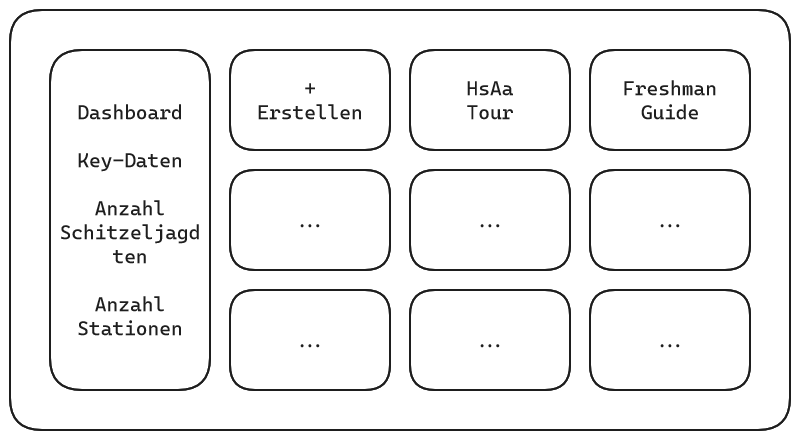
\includegraphics[width=1\textwidth]{images/wireframing/PrAr_Scavhunt_Wireframing-2.1.png}
  \caption{Skizze Dashboard des Hunt-Editors}
  \label{fig:wireframing-frontend-hunt-editor-3}
\end{figure}

Dies ist ein Wireframe, das relativ am Anfang der Entwicklungsphase erstellt wurde. Hier wurde ein Grid-Layout verwendet, um die Schnitzeljagd darzustellen. An der Seite befindet sich eine Sidebar, in der verschiedene Schlüsseldaten abgelesen werden können. Da es aber aufgrund der Architekturänderungen keine Stationen mehr gibt, fällt diese Information weg. Das Grid-Layout soll jedoch beibehalten werden.

\begin{figure}[H]
  \centering
  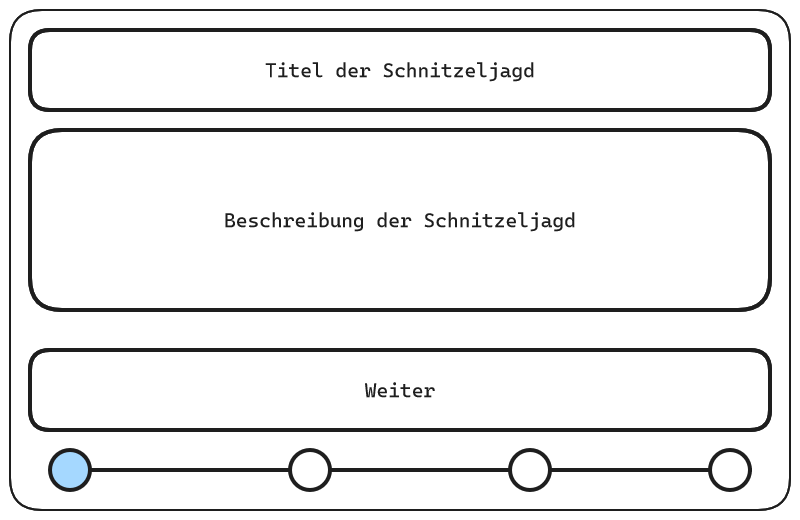
\includegraphics[width=1\textwidth]{images/wireframing/PrAr_Scavhunt_Wireframing-2.2.png}
  \caption{Skizze für Eingabe von Basisdaten im Hunt-Editor}
  \label{fig:wireframing-frontend-hunt-editor-4}
\end{figure}

Hier wird nun der Prozess der Erstellung einer Schnitzeljagd beschrieben, wobei uns die Verwendung eines Fortschrittsbalkens gefallen hat, der den aktuellen Stand der Erstellung anzeigt. Auch die Eingabe von Titel und Beschreibung sollte später so übernommen werden. 

\begin{figure}[H]
  \centering
  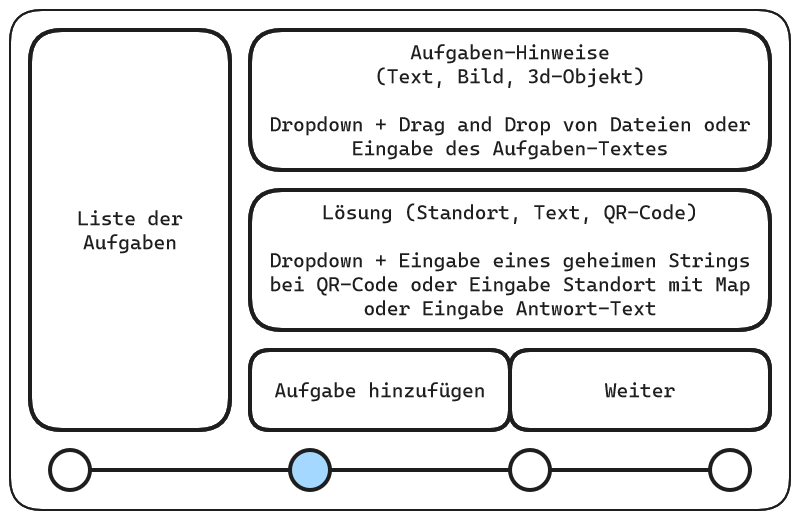
\includegraphics[width=1\textwidth]{images/wireframing/PrAr_Scavhunt_Wireframing-2.3.png}
  \caption{Skizze für Anlegen von Aufgaben im Hunt-Editor}
  \label{fig:wireframing-frontend-hunt-editor-5}
\end{figure}

Nun kommt der schwierigste Teil, die Erstellung und Bearbeitung der Aufgaben in einer Schnitzeljagd. Hier war zunächst der Ansatz, auf der linken Seite eine Tabelle mit den Aufgaben zu führen. Durch Anklicken der entsprechenden Zeile wird dann auf der rechten Seite die Aufgabe und die Lösung angezeigt. Hier gibt es auch noch den Aufgabentyp "3D-Objekt", der am Ende nicht übernommen wurde. 

\begin{figure}[H]
  \centering
  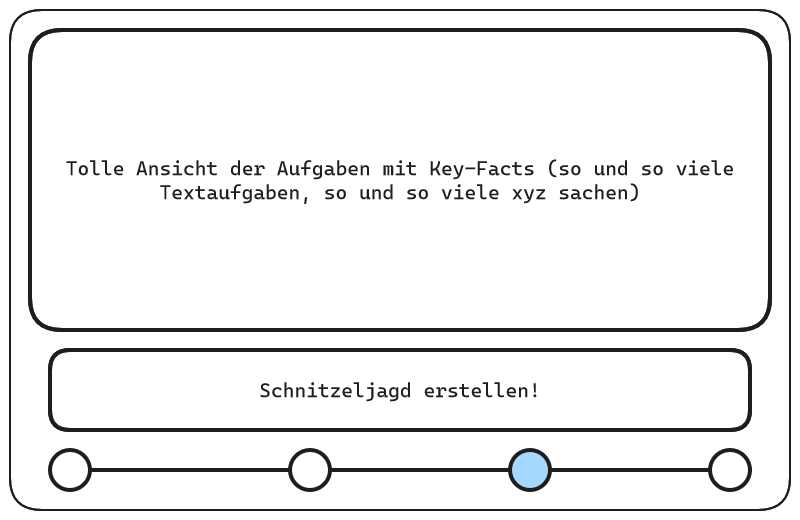
\includegraphics[width=1\textwidth]{images/wireframing/PrAr_Scavhunt_Wireframing-2.4.png}
  \caption{Skizze zur Übersicht einer Schnitzeljagd im Hunt-Editor}
  \label{fig:wireframing-frontend-hunt-editor-6}
\end{figure}

Dieses Wireframe zeigt am Ende noch einmal alle wichtigen Informationen der Schnitzeljagd im Überblick. Dieses Konzept hat uns gut gefallen. 

\begin{figure}[H]
  \centering
  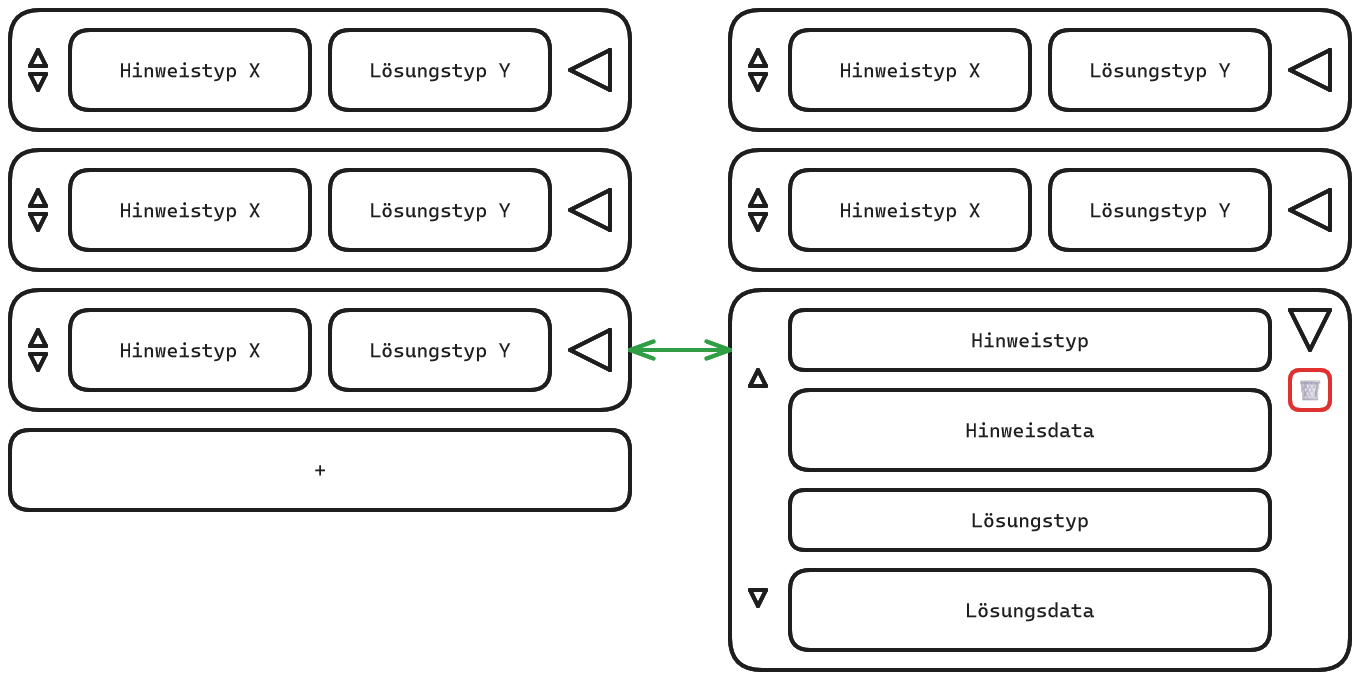
\includegraphics[width=1\textwidth]{images/wireframing/PrAr_Scavhunt_Wireframing-3.png}
  \caption{Skizze zur Auflistung von Aufgaben im Hunt-Editor}
  \label{fig:wireframing-frontend-hunt-editor-7}
\end{figure}

Da die seitliche Liste in Abbildung \ref{fig:wireframing-frontend-hunt-editor-5} für die Darstellung der Aufgaben auf mobilen Endgeräten ungeeignet ist, haben wir uns für den Ansatz in Abbildung \ref{fig:wireframing-frontend-hunt-editor-7} entschieden. Hier werden die Aufgaben nacheinander angezeigt und ihre Reihenfolge kann über die Pfeiltasten verändert werden. Um die Aufgaben zu bearbeiten, können diese über den Button auf der rechten Seite aufgeklappt und wieder zugeklappt werden. Im aufgeklappten Zustand befindet sich jeweils ein Dropdown für Aufgabe und Lösung sowie Eingabefelder / FileUpload oder eine Map-Integration für den Standort als Lösung. 

\section{Participation Web-App}

\subsection{Übersicht}

Über die Participation Web App kann sich ein Teilnehmer für eine Schnitzeljagd anmelden. Dazu startet er die Anwendung und gelangt auf eine Willkommensseite. Hier kann er sehen, wie viele Teilnehmer und wie viele Teilnahmen es insgesamt gibt. Um an einer Schnitzeljagd teilzunehmen, kann der Teilnehmer eine E-Mail an den Organisator schreiben. Wenn er daraufhin einen Einladungslink für eine Schnitzeljagd erhält, muss er dort nur noch einen Benutzernamen und ein Passwort auswählen. Mit diesem Benutzernamen und Passwort loggt er sich in das im Kapitel \ref{subsec:swentwurf:hunt-game} beschriebene Hunt-Game ein.

\subsection{Wireframing}

\begin{figure}[H]
  \centering
  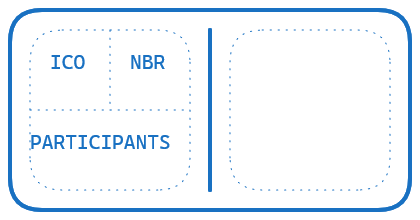
\includegraphics[width=1\textwidth]{images/PrAr_Scavhunt_Wireframing_Participant_1.png}
  \caption{Skizze zur Anzeige von Statistiken in der Participation Web-App}
  \label{fig:wireframing-frontend-participant-1}
\end{figure}

Um auf der Startseite der Participation Web-App interessante Statistiken anzeigen zu können, musste ein Konzept gefunden werden, wie diese ansprechend dargestellt werden können. Auf der linken Seite sollte die Anzahl aller Teilnehmer und auf der rechten Seite die Anzahl aller Beteiligungen dargestellt werden. Diese Informationen werden durch eine vertikale Trennlinie getrennt, um die verschiedenen Statistiken klar voneinander abzugrenzen.

\begin{figure}[H]
  \centering
  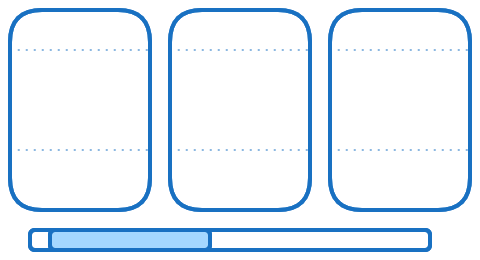
\includegraphics[width=1\textwidth]{images/PrAr_Scavhunt_Wireframing_Participant_2.png}
  \caption{Skizze zur Benachrichtigung eines Organisators in der Participation Web-App}
  \label{fig:wireframing-frontend-participant-2}
\end{figure}

Der Teilnehmer soll auch die Möglichkeit haben, einen Organisator um einen Einladungslink zu bitten. Dazu wurde das Wireframe erstellt, in dem die Organisatoren als Karten dargestellt werden. Hier kann auf mobilen Geräten durch horizontales Wischen zwischen den Organisatoren gewählt werden. 
\section{Hunt-Game Web-App} \label{subsec:swentwurf:hunt-game}

\subsection{Übersicht}
Beim Start der Anwendung sieht der Teilnehmer eine Sammlung von Bildern der Hochschule Aalen, darunter eine kleine Zeitleiste, die den Entwicklungsprozess der Projektarbeit beschreibt. Um an einer Schnitzeljagd teilnehmen zu können, muss sich der Teilnehmer mit dem gewählten Benutzernamen und Passwort der Participation Web-App anmelden. Anschließend wird ihm eine Übersicht aller Schnitzeljagden angezeigt, für die er sich registriert hat. Hierbei wird zwischen \textit{Ongoing, Complete} und \textit{Expired} unterschieden, was durch den aktuellen Teilnahme-Status bestimmt wird. Wählt er eine gültige Schnitzeljagd aus, startet der Spielablauf. 

\subsection{Spielablauf} \label{cha:swentwurf:spielablauf}

Abbildung \ref{fig:hunt_game_spielablauf} stellt den Spielablauf als UML-Programmablaufplan dar. 

\begin{figure}[H]
  \centering
  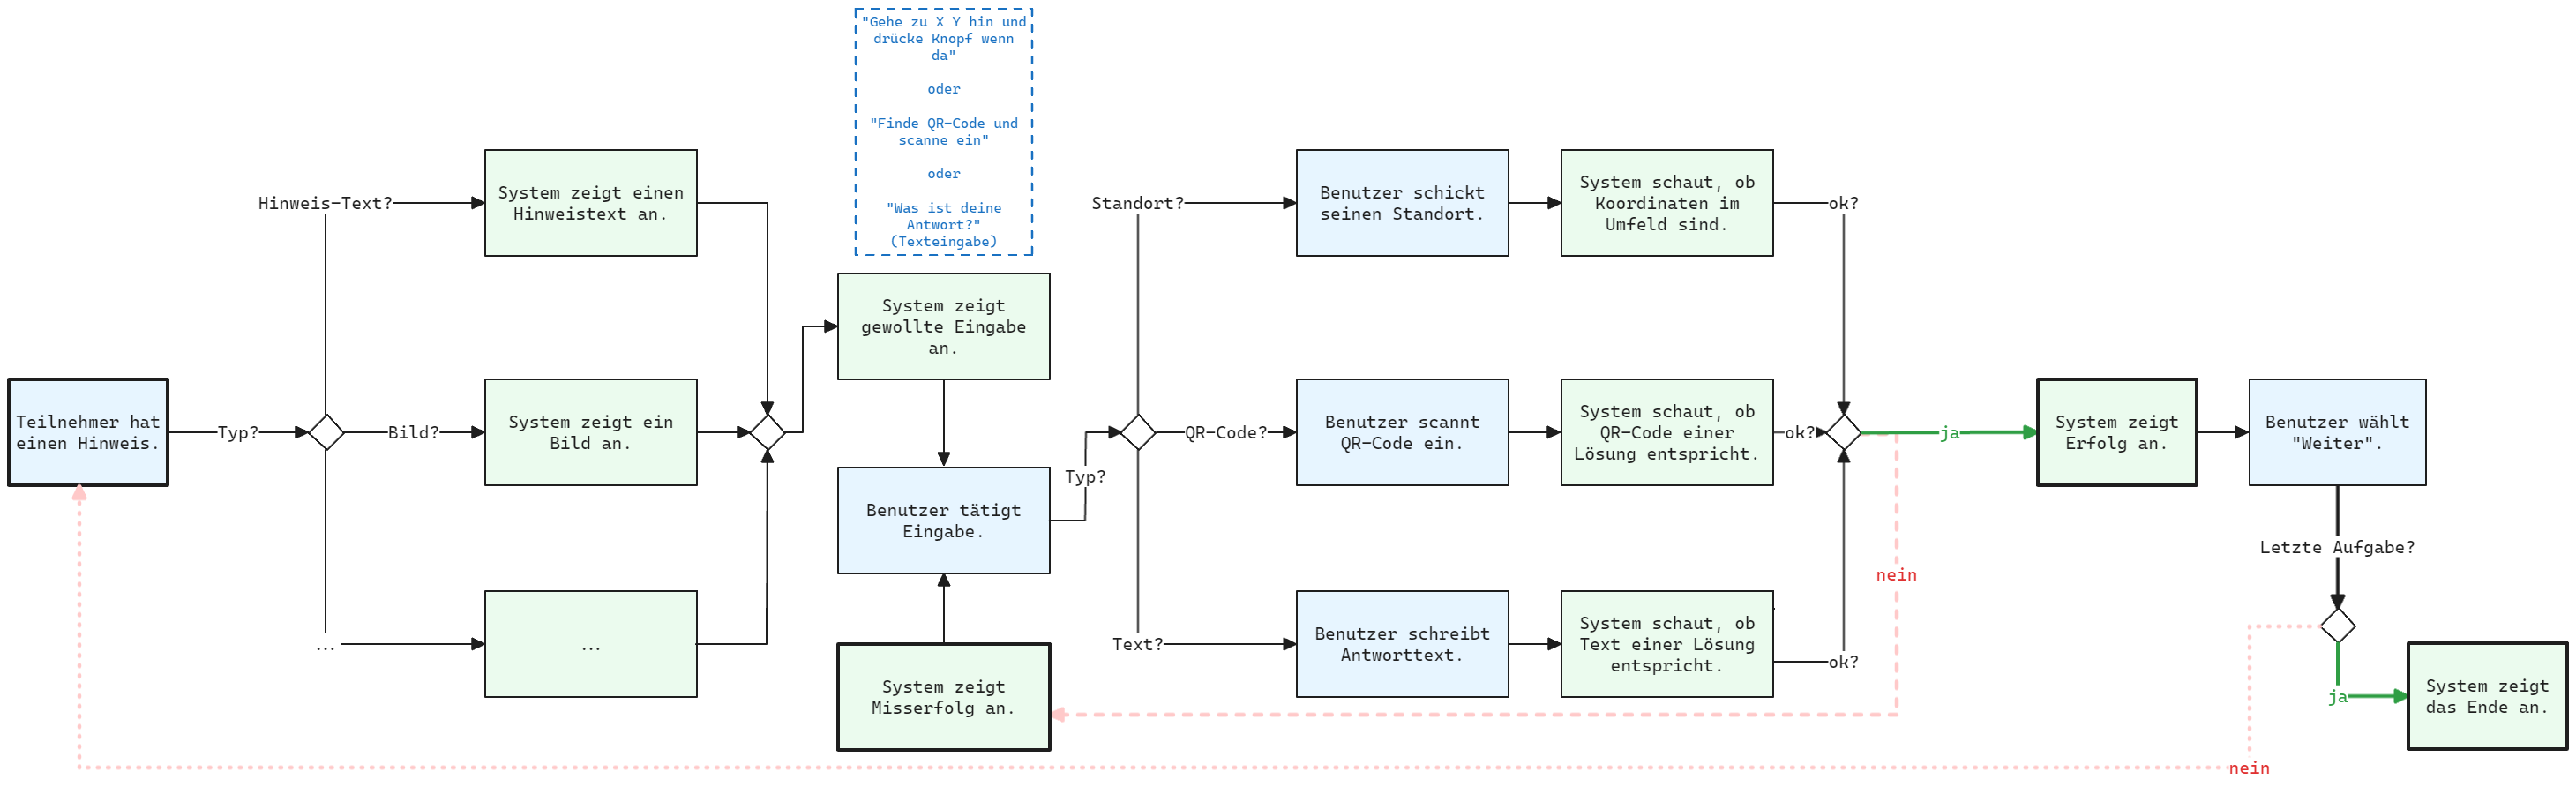
\includegraphics[width=\textwidth]{images/PrAr_Spielablauf.png}
  \caption{Skizze Spielablauf als UML-Programmablaufplan}
  \label{fig:hunt_game_spielablauf}
\end{figure}

Nachdem der Teilnehmer eine gültige Schnitzeljagd ausgewählt hat, beginnt der eigentliche Spielablauf. Zu Beginn wird dem Teilnehmer der aktuelle Hinweis präsentiert, der ihn zur nächsten Station oder Aufgabe führen soll. Die Hinweise sind in zwei Arten unterteilt: Text und Bild. Bei einem Texthinweis wird dem Teilnehmer ein beschreibender Text angezeigt, der Informationen oder Anweisungen zur nächsten Station enthält. Bei einem Bildhinweis wird stattdessen ein Bild angezeigt, das visuelle Hinweise oder Details enthält, die zur Lösung der Aufgabe beitragen.

Unter dem Hinweis befindet sich ein Button, über den der Teilnehmer seine Lösung einreichen kann. Es gibt drei verschiedene Lösungstypen, die je nach Aufgabe variieren:
\begin{itemize}
    \item \textbf{Textlösung}: Der Teilnehmer gibt seine Lösung in ein Textfeld ein. Dies kann z.B. ein gesuchtes Wort, ein Satz oder eine Zahlenkombination sein.

    \item \textbf{QR-Code}: Bei Aufgaben, die einen QR-Code erfordern, wird die Kamera des Gerätes aktiviert, um den QR-Code einzuscannen. Dieser QR-Code kann an verschiedenen Stellen versteckt sein und enthält die notwendigen Informationen oder Anweisungen, um zum nächsten Hinweis zu gelangen.

    \item \textbf{Location}: Wenn die Lösung in Form eines geographischen Ortes zur Verfügung gestellt werden soll, wird der Teilnehmer aufgefordert, den Zugriff auf den Ort zu erlauben. Der Browser ermittelt dann die aktuellen GPS-Koordinaten des Geräts und prüft, ob diese mit der erwarteten Lösung übereinstimmen.
\end{itemize}

Der Spielablauf wiederholt sich, bis alle Aufgaben gelöst sind. Bei den Lösungstypen Text und Ort erhält der Teilnehmer zusätzlich Hinweise, wenn seine Lösung nicht korrekt ist. Diese Hinweise besagen, dass die Lösung fast richtig ist, aber noch angepasst werden muss. Dies soll den Teilnehmer ermutigen und ihm die Möglichkeit geben, seine Antwort zu verbessern.




